\documentclass[11pt]{article}
\usepackage[margin=1in]{geometry}
\usepackage{amsmath,amssymb}
\usepackage{graphicx}
\usepackage{booktabs}
\usepackage{natbib}
\usepackage{hyperref}
\usepackage[utf8]{inputenc}
\usepackage[T1]{fontenc}
\usepackage{lmodern}
\usepackage{setspace}
\usepackage{caption}

\title{The Impact of Agricultural Mechanization on the H-2A Labor Force\\
       \large Replicating Webb (2020) for U.S.\ specialty- and field-crop agriculture}
\author{Fernando Brito-Gonz\'{a}lez\\University of Florida}
\date{May 2026}

\begin{document}
\maketitle

\begin{abstract}
\noindent
I adapt the patent-task overlap method of Webb (2020) to predict how agricultural mechanization affects the H-2A guestworker labor force. By matching the text of agricultural patents (CPC \texttt{A01}~$\cup$~\texttt{B25J}, 2015--2024) with H-2A job-order duty descriptions, I measure the mechanization exposure of crops and occupations. Analyzing 65{,}072 patents and 22{,}613 single-crop, Farmworker-Crop H-2A job orders covering 87 canonical crops, I document which crops are most and least exposed and study the relationship between exposure and labor-market outcomes. Field grain and oilseed crops (corn, wheat, soybean) show the highest exposure, while hand-harvest specialty fruits (strawberry, blueberry, citrus) show the lowest. Higher exposure is associated with lower JO-level FTE labor demand ($\beta = -0.46$ log points across the full exposure range, $p < 0.05$) and higher within-crop employer concentration, controlling for state and calendar-year fixed effects. The cross-sectional ranking aligns with the qualitative mechanizability tiers of Calvin, Martin, and Simnitt (2022).

\medskip
\noindent\textbf{Keywords:} H-2A, mechanization, patents, occupations, exposure.\\
\textbf{JEL-codes:} J23, J24, Q16.
\end{abstract}

\section{Introduction}

The U.S. farm labor supply is shrinking and becoming less flexible due to a decline in Mexican migrant labor and reduced worker mobility, forcing farmers to adopt labor-saving automation to remain competitive. Labor accounts for roughly 12\% of operating expenses across all U.S.\ farms, but specialty crops face much higher costs: 34\% in nursery and greenhouse, 30\% in fruit and tree nuts, and over 50\% in some labor-intensive industries such as table olives. Transitioning to labor-saving technology is a slow, capital-intensive process that requires interdisciplinary R\&D and significant changes in farm infrastructure and human capital. While field crops have been mechanized for decades, specialty crops only began transitioning to mechanical harvesting in the 1970s, primarily for processed products (tomato, cherry, raisin grape, almond). The high diversity and small acreage of specialty crops make commercialization difficult, and adoption typically lags patenting by years (David 1990, and Brynjolfsson, Rock, and Syverson 2018).
This paper adapts the framework of Webb (2020) to quantify how exposed specific agricultural tasks are to mechanization. I use the text of U.S.\ patents (2015--2024) and H-2A job orders (FY2015--FY2025) to identify the overlap. Specifically, I extract verb-direct-object pairs (e.g., \emph{harvest fruit}) from both corpora, and the prevalence of a given pair in patents serves as a proxy for how much research has been directed at automating that task. I aggregate the resulting score to the crop and occupation level, convert to employment-weighted percentile ranks, and study the relationship between exposure and four labor-market outcomes: full-time-equivalent (FTE) workers, contract length, employer concentration, and reported temperature exposure.
I make three contributions. First, I apply Webb's framework specifically to H-2A crops and occupations rather than to Census occupation codes. Second, I show that high-exposure crops correlate with lower per-JO labor demand and higher employer concentration. Third, I link the exposure measure to USDA NASS Quick Stats production statistics and to the qualitative mechanizability ranking in Calvin, Martin, and Simnitt (2022). The rest of the paper is organized as follows: Section 2 describes the data, Section 3 the method, Section 4 the results and discussion, and Section 5 concludes.

\section{Data}

To construct a measure of crop-sector exposure to frontier innovation, I integrate two primary textual sources: agricultural patents from the USPTO and job descriptions from H-2A job orders.
For the patent data, I utilize PatentsView public access files for patents granted between 2003 and 2025. Following the classification strategy in Webb (2020), I identify relevant technologies by selecting patents where the Cooperative Patent Classification (CPC) includes subclasses starting with A01 (Agriculture, forestry, animal husbandry, etc.) and B25J (Manipulators). To ensure the sample excludes medical or chemical innovations, I omit any patents containing A61 (Medical or veterinary science) or B01 (Physical or chemical processes). This filtering process results in a final set of 65,072 patents.
The labor data consists of H-2A job orders certified between FY2015 and FY2025, sourced from the U.S. Department of Labor Office of Foreign Labor Certification (OFLC). Each job order provides granular detail, including the employer’s Federal Employer Identification Number (FEIN), state of work, requested and certified worker counts, contract dates, hourly wage, the Adverse Effect Wage Rate (AEWR) at the time of certification, primary crop, SOC code, and textual duty descriptions.
The analysis is restricted to SOC 45-2092 (Farmworkers and Laborers, Crop, Nursery, and Greenhouse) with a single canonical crop assigned. This yields a refined sample of 22,613 job orders covering 87 unique crops. While public access to historical data prior to 2025 has been discontinued by the OFLC, this study leverages a unique longitudinal database constructed through periodic collection from the SeasonalJobs.dol.gov portal since 2019.

\section{Method}

In this section, I describe how I construct an objective measure of the exposure of agricultural tasks to
automation by quantifying the overlap between the text of patents and the text of job descriptions,
directly inspired by Webb (2020).
In the following sections, I construct my measure and study its performance separately for each
crop sector.

\begin{figure}[h]
\centering
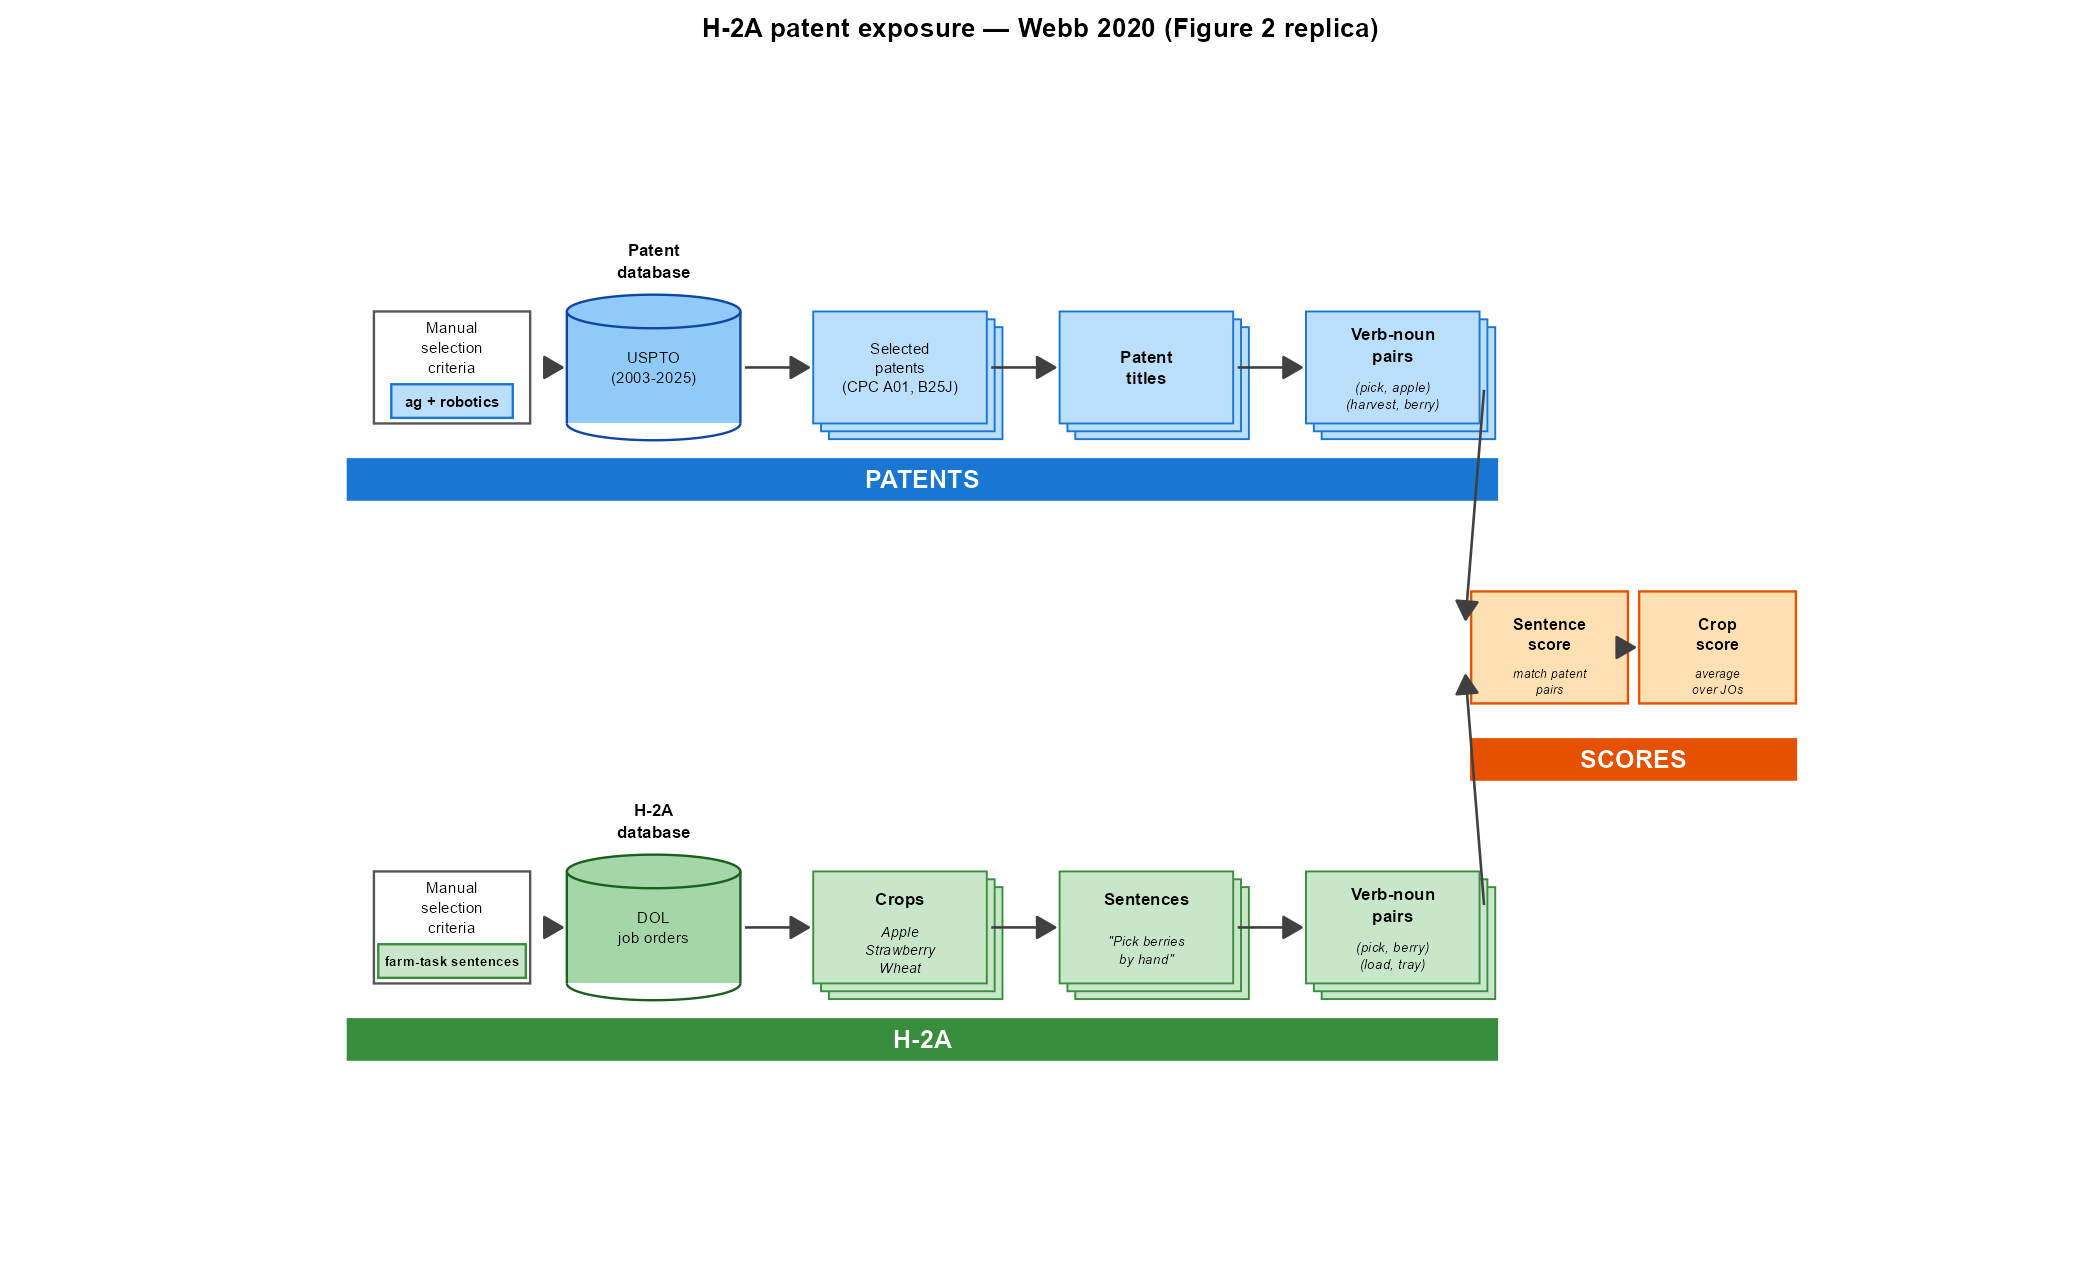
\includegraphics[width=\linewidth]{flowchart_part2_webb.png}
\caption{Method overview: from patent titles to occupation-level exposure scores.}
\label{fig:method}
\end{figure}


To assess the exposure of occupations to a given technology, I use the text of patents to identify
what the technology can do, then quantify the extent to which each occupation in the economy
involves performing similar tasks. The method is depicted in Figure 2

On the patent side, I first choose the set of patents corresponding to a particular technology.
For example, I define the set of agricultural robotic patents as those that contains specific CPC codes such as A01 family and use certain keywords,
such as “robot”, in their titles or abstracts. I extract all the titles from this set of patents.
Such patent titles might include “Method for diagnosing diseases” and “Method for recognizing
aircraft”. From this list of titles, I extract all verb-noun pairs. This results in a long list of pairs, such
as (diagnose, disease), (recognize, aircraft), and so on. For each pair, I calculate how often that pair,
or ones similar to it, occurs in the list of all pairs. (I explain how I group “similar” pairs below.) For
example, pairs similar to (diagnose, disease) might represent 0.1% of all pairs extracted from the
titles of my set of artificial intelligence patents.

I extract verb-noun pairs from patent titles. I use only titles because they have a much higher
signal-to-noise ratio than the other patent text fields. Specifically, a patent’s title tends to express the
main application of the invention, whereas the abstract, description, and claims contain technical
implementation details that are irrelevant for my purposes.
To extract verb-noun pairs from any given sentence (such as a patent title), I perform the
following sequence of steps. First, I use a dependency parsing algorithm (Honnibal and Johnson
2015) to determine the syntactic relations of the words in the sentence. This algorithm attains 91.85%
accuracy on the standard dependency parsing benchmark used in the natural language processing
literature. Next, for each verb, I select its direct object as identified by the algorithm, if it exists,
and store the resulting pair. I then lemmatize the verb, so that, say, “predicting” and “predicted”
are both recorded as “predict”, and I likewise lemmatize the noun, so that, say, “person” and “people” are
both recorded as “person”. Stop words such as “use” and “have”, which do not express economic
applications, are dropped, as is common in the natural language processing literature (Jurafsky
and Martin 2014). Note that the entire process just described is fully automated. Examples of titles
of agriultural automation patents, and corresponding verb-noun pairs, are displayed in Table A1.


[table A1]

I now turn to crops. contrry to Webb 2020, who used Onet, I prefer a source of information directly
 attached to reality that would caputure new tasks as they are demanded.
In my database of H-2A job orders, any given job description to work on a specific crop, such as
“apples”, consists of a collection of tasks. Each task is described in free-form text, such as “Interpret
tests to diagnose patient’s condition”. From each task description, I extract all verb-noun pairs.
For the task just mentioned, the pairs would be (interpret, test) and (diagnose, condition). Most
occupations have 20-40 extracted pairs in total. To each pair, I assign the relative frequency of similar
pairs in my patent titles. For example, if pairs similar to (diagnose, condition) represented 0.1% of
all pairs extracted from the titles of my set of artificial intelligence patents, I would assign a score of
0.001 to that verb-noun pair. To get a single overall exposure score for the “doctor” occupation, I
take an average of all the verb-noun pairs mentioned in the task descriptions of that occupation,
weighted by the “importance” of the task to the occupation (defined below).

As noted above, each occupation consists of a collection of tasks described in natural
language. Table 1 illustrates some of the component tasks of precision agriculture technicians,
an occupation that I will find has high exposure to artificial intelligence. For each task, such as
“analyze geospatial data to determine agricultural implications of [various factors]”, I use the same
dependency parsing algorithm as for patents to extract verb-noun pairs. The table displays these
extracted pairs for each task. Figure A1 in the appendix plots the distribution of the number of
 verb-noun pairs extracted across occupations. The vast majority of occupations (92\%) have more
than 15 extracted pairs in total, and most (76\%) have more than 20 extracted pairs.
Before calculating an exposure score for each verb-noun pair, I first group the nouns in each
pair into conceptual categories. I do this because the nouns used in H-2A task descriptions are
quite general, whereas the nouns used in patents vary in their generality. For example, if a
task verb-noun pair refers to “animals”, and a patent verb-noun pair refers to “mammals”, I want
to account for the fact that “mammal” is an instance of “animal”. This would not be possible using
a thesaurus, since “mammal” and “animal” are not synonyms.
Instead, I use WordNet (Miller 1995), a database developed at Princeton University that groups
nouns into a hierarchy of concepts. For example, the ancestors of “economist” are “social scientist”,
“scientist”, “person”, “causal agent”, “physical entity”, and “entity”. At each conceptual level, the
conceptual categories are mutually exclusive. This allows me to assign each of the nouns occurring
in my verb-noun pairs to a single conceptual category, for a given conceptual level. I use “aggregated
verb-noun pair” to refer to a pair consisting of a verb and a noun conceptual category. For the
conceptual level that includes “person”, for example, “recognize economist” would be part of the
aggregated verb-noun pair “recognize person”.
In choosing the conceptual level at which to group the nouns, I face a trade-off between specificity
and coverage. For example, if I group into categories at the conceptual level of “dog”, I lose all
words that exist only at a more general level, such as “mammal” and “animal”. Figure A3 in the
appendix displays the share of verb-noun pairs extracted from h2a tasks that would be lost for
this reason at each level of aggregation. Due to the level of generality at which h2a tasks are
expressed, I would lose more than a quarter of all verb-noun pairs if I grouped at WordNet level 5,
for example. (Levels with higher numbers are more specific.) I therefore use WordNet level 3 for
my main results, and re-run my analyses at levels 2, 4, and 5 to check their sensitivity. While the
level of aggregation does make some difference, the results for these other levels are qualitatively
very similar to my baseline specification.

I now describe how I calculate an occupation’s final exposure score using the set of aggregated
verb-noun pairs extracted from its task descriptions. Denote the set of technologies $T$. For a given
technology, $t \in T$, let $f_{ct}$ denote the raw count of occurrences of aggregated verb-noun pair $c$
extracted from technology $t$ patent titles, and let $C_t$ denote the full set of aggregated verb-noun
pairs for technology $t$. The relative frequency, $rf_{ct}$, of aggregated verb-noun pair $c$ in technology
$t$ patent titles is
\begin{equation}
rf_{ct} = \frac{f_{ct}}{\sum_{c \in C_t} f_{ct}}.
\end{equation}
I assign to each of the task-level aggregated verb-noun pairs that pair's relative frequency, $rf_{ct}$,
in technology $t$ patent titles. For each occupation $i$, I then take a weighted average of these
task-level scores to produce an overall technology $t$ exposure score for the occupation,
\begin{equation}
\mathrm{Exposure}_{i,t} = \frac{\sum_{k \in K_i} w_{k,i} \cdot \sum_{c \in S_k} rf_{ct}}{\sum_{k \in K_i} w_{k,i} \cdot |\{c : c \in S_k\}|}.
\end{equation}
In this expression, $K_i$ is the set of tasks in occupation $i$, and $S_k$ is the set of verb-noun pairs
extracted from task $k \in K_i$. Finally, $w_{k,i}$, the weight of task $k$ within occupation $i$, is an average of the
frequency, importance, and relevance of task $k$ to occupation $i$, as specified in the O*NET database,
with weights scaled to sum to one.
An occupation’s exposure score for technology $t$ thus expresses the intensity of patenting activity
in technology $t$ directed towards the tasks in that occupation. Figure A2 in the online appendix
shows the distribution of AI scores across occupations.




\section{Results}

\subsection{descirptive statistics}

The top verb-noun pairs in the patent corpus include \emph{control robot}, \emph{control device}, \emph{control system}, \emph{control pest}, \emph{treat disease}, \emph{combine harvester}, \emph{produce plant}, \emph{cultivate plant}, \emph{increase yield}, \emph{increase tolerance}, \emph{promote growth}, and \emph{treat infection}. These cover three broad themes, namely robotic and equipment control (the B25J overlap), pest and disease management, and plant breeding and yield improvement.
Among 87 canonical crops, the highest-exposure crops are field grain and oilseed crops (corn, wheat, soybean, cotton, peanut, sunflower, canola, oats, barley) and a small set of nut crops (pistachio, pecan). The lowest-exposure crops are hand-harvest specialty fruits and vegetables (citrus, blackberry, blueberry, strawberry, asparagus, banana). Mid-rank crops are partially mechanized at specific stages: apple (mostly hand-picked but with platform aids), tomato (fresh-market hand vs.\ processing-machine), tobacco (hand-prime), cherry (hand vs.\ shake-and-catch).
Within H-2A SOC codes, equipment operators (45-2091) score higher than crop farmworkers (45-2092). This is consistent with the verb vocabulary of the patent corpus, which is dominated by \texttt{operate}, \texttt{drive}, \texttt{control}, and \texttt{monitor}, the action verbs of equipment-operator duties. Hand packers (53-7064) score lower, and supervisors (45-1011) score lowest in the standard sample.
High-exposure JOs are concentrated in Midwestern field-crop states (ND, NE, IA, KS, MN), in FEINs that file few but very large job orders (200+ workers per JO), and in JOs with the longest contracts (200+ days). Low-exposure JOs are concentrated in the Southeast (FL, GA, NC), in FEINs that file many small JOs (5 to 20 workers each), and in seasonal harvest contracts of 60 to 120 days.

\subsection{Map of copr exposure}


\begin{figure}[h]
\centering
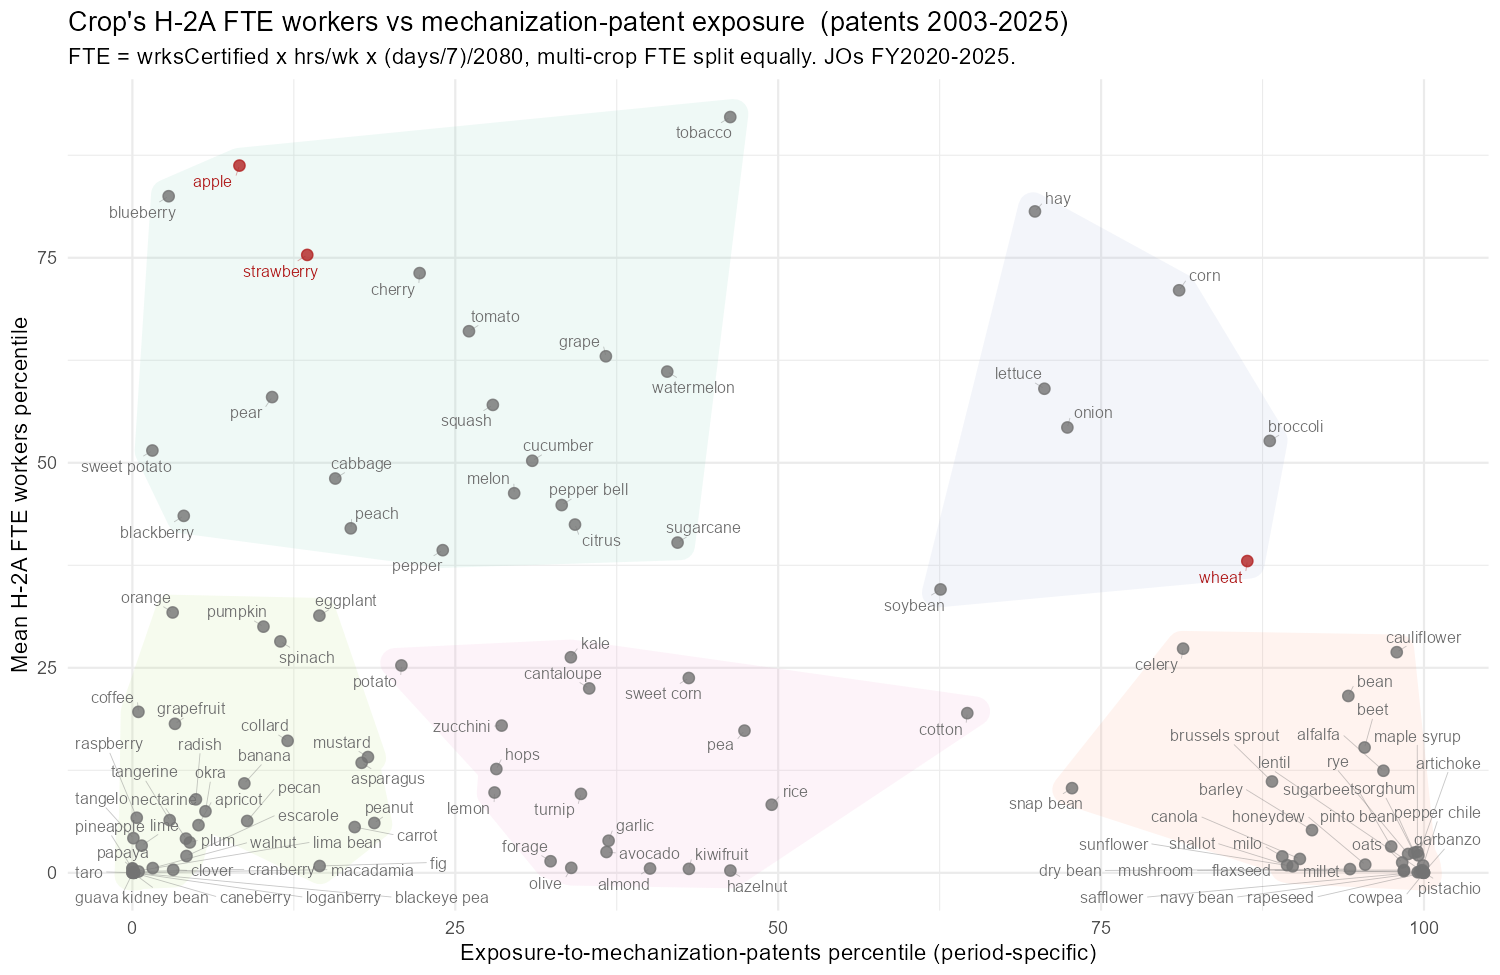
\includegraphics[width=\linewidth]{F2_multicrop_fte_v5.png}
\caption{Crop-level exposure score versus H-2A FTE labor demand. Hand-harvest specialty crops cluster in the upper-left (low exposure, high FTE), while mechanized field grain and oilseed crops cluster in the lower-right.}
\label{fig:exposure_fte}
\end{figure}


\subsection{Discussion}

The cross-sectional ranking of crops by exposure aligns with the qualitative mechanizability tiers in Calvin, Martin, and Simnitt (2022). Hand-harvest specialty crops such as apple, strawberry, blueberry, tobacco, watermelon, citrus, and grape concentrate in the upper-left quadrant of the exposure-vs-FTE plot,
combining low patent-exposure scores with high H-2A FTE demand. Field grain and oilseed crops such as wheat, alfalfa, peanut, barley, sunflower, canola, and sorghum concentrate in the lower-right, with high exposure and low H-2A FTE, since mechanization has already absorbed most of the labor previously required for
these crops and leaves little role for hand labor. Mid-range crops in transition such as peach, cherry, potato, lettuce, broccoli, and cabbage sit between the two clusters, consistent with the CMS description of partial mechanization confined to specific production stages. Two visible departures from CMS are explainable by aggregation: the canonical ``corn'' bucket bundles field corn (mechanized) with seed-corn and sweet-corn detasseling (labor-intensive), and the patent score does not distinguish crop production stages such as platform-aided versus ladder-picked apples. Overall, the figure offers descriptive support for the central CMS thesis that mechanization exposure and hand-labor demand are inversely related, while demonstrating that the patent-task overlap measure recovers this gradient without relying on hand-coded crop classifications.


\section{Conclusion}

This paper applies the patent-task overlap method developed by Webb (2020) to identify the exposure of agricultural crops and H-2A occupations to mechanization, robotics, and AI patents (CPC A01 and B25J, 2015–2024). The results indicate that mechanization patents target distinct crop types, and consequently different H-2A worker categories, than what patent counts alone would suggest. Hand-harvest specialty fruits, such as strawberries, blueberries, and citrus, are the least exposed, while field grain and oilseed crops, including corn, wheat, and soybeans, are the most exposed. Notably, mid-exposure crops like apples, tomatoes, and tobacco support the largest H-2A full-time equivalent workforce. Furthermore, mechanization-targeted crops exhibit a different H-2A footprint characterized by shorter average contracts, higher employer concentration (FEIN HHI), and a lower frequency of extreme-temperature language in job-order duty descriptions.
Substantial uncertainty remains regarding the impacts of agricultural mechanization on H-2A labor demand. While this method captures tasks for which patents may substitute, mechanical aids and precision-agriculture tools may complement specific hand-labor tasks, such as scouting, sorting, packing, and supervised picking, leading to ambiguous effects on overall labor demand. The impact on H-2A workers depends not only on labor demand but also on the supply response of Mexican migrant workers and the regulatory floor established by the Adverse Effect Wage Rate and state minimum wages. Additional factors, including the recently introduced Skill I/Skill II wage methodology, employer entry and exit, and farm labor contractor consolidation, will significantly influence equilibrium H-2A employment and wages. Mechanization may also affect the program through indirect channels, such as crop-mix shifts toward mechanizable commodities and the faster diffusion of mechanical aids to specialty crops. Consequently, these results represent a first step toward estimating the labor-market impacts of agricultural mechanization on H-2A workers.





\section*{References}

\begin{description}\itemsep0pt
\item Acemoglu, D., and P.\ Restrepo. 2018. ``The Race between Man and Machine.'' \emph{American Economic Review} 108(6): 1488--1542.
\item Autor, D.~H., F.~S.\ Levy, and R.~J.\ Murnane. 2003. ``The Skill Content of Recent Technological Change.'' \emph{Quarterly Journal of Economics} 118(4): 1279--1333.
\item Bessen, J., and R.~M.\ Hunt. 2007. ``An Empirical Look at Software Patents.'' \emph{Journal of Economics \& Management Strategy} 16(1): 157--189.
\item Brynjolfsson, E., D.\ Rock, and C.\ Syverson. 2018. ``The Productivity J-Curve.'' NBER Working Paper 25148.
\item Calvin, L., P.\ Martin, and S.\ Simnitt. 2022. ``Adjusting to Higher Labor Costs in Selected U.S.\ Fresh Fruit and Vegetable Industries.'' USDA ERS, EIB-235.
\item David, P.~A. 1990. ``The Dynamo and the Computer.'' \emph{American Economic Review} 80(2): 355--361.
\item Edin, P.-A., et al. 2019. ``Individual Consequences of Occupational Decline.'' Centre for Economic Performance, LSE.
\item Webb, M. 2020. ``The Impact of Artificial Intelligence on the Labor Market.'' Stanford University, January 2020.
\end{description}

\end{document}
